\documentclass[11pt,a4paper]{article}
\usepackage[utf8]{inputenc}
\usepackage[T1]{fontenc}
\usepackage{graphicx}
\usepackage{amsmath}
\usepackage{natbib}
\usepackage{hyperref}
\usepackage{booktabs}
\usepackage{siunitx}
\usepackage{longtable}
\usepackage{lineno}
\usepackage[margin=1in]{geometry}
\usepackage{multirow}
\usepackage[table]{xcolor}
\usepackage{threeparttable}

% Line numbers for review
\linenumbers

\title{Energy System Constraints on Industrial Decarbonization: Why Grid Capacity Favors Hydrogen for Petrochemicals}

\author{
Jinsu Park\textsuperscript{1,*} \\
\small \textsuperscript{1}PLANiT Institute, Seoul, South Korea \\
\small \textsuperscript{*}Corresponding author: jinsu@planit.institute
}

\date{}

\begin{document}

\maketitle

\begin{abstract}
Global industrial decarbonization efforts increasingly rely on Marginal Abatement Cost Curve (MACC) analysis to rank technology pathways, yet this partial equilibrium approach systematically ignores whether national energy systems can accommodate aggregate sectoral demands---potentially rendering cost-competitive pathways physically infeasible. We develop a facility-level MACC model for South Korea's petrochemical sector (248 facilities, 66.2 MtCO\textsubscript{2}/year, 13\% of national emissions) that explicitly quantifies electricity and hydrogen demands across six scenarios combining production pathways (business-as-usual growth, 25\% capacity restructuring, 40\% restructuring) with competing technology routes (hydrogen-fueled steam crackers vs. electrically-heated crackers).

Our analysis reveals cost parity masking system-level divergence. Hydrogen and electricity pathways show nearly identical cumulative costs (\$31.4 billion vs. \$33.3 billion, 6\% difference), yet the electricity pathway requires 164.5 TWh annually by 2050---consuming 97\% of Korea's 2036 renewable electricity target before accounting for competing sectoral demands. In contrast, the hydrogen pathway requires 7.7 Mt H\textsubscript{2} annually---only 28\% of Korea's planned 2050 supply capacity, achievable through dedicated off-grid infrastructure and imports. Even aggressive capacity restructuring (40\% reduction) cannot resolve the electricity pathway's binding grid constraint, requiring 86 TWh (51\% of renewable target).

Grid capacity, not technology cost, emerges as the binding constraint for industrial decarbonization. These findings validate hydrogen infrastructure as necessary rather than optional for heavy industry, with implications extending to EU, Japan, and industrialized economies facing similar resource-constrained grids. Technology-system co-optimization must replace partial equilibrium analysis to avoid systematically misleading industrial climate policy.
\end{abstract}

\noindent \textbf{Keywords:} Industrial decarbonization, petrochemicals, MACC methodology, energy system constraints, hydrogen economy, electrification, South Korea, renewable energy

\newpage

\section{Introduction}

Industrial decarbonization has emerged as a critical frontier in global climate policy, with pathways increasingly centered on electrification powered by renewable energy \citep{IEA2023,Kaufman2024}. Recent studies emphasize electrifying high-temperature industrial processes---including steel, cement, and petrochemicals---to eliminate fossil fuel combustion emissions \citep{Kloo2024,Diesing2025}. This "electrify everything" paradigm assumes national grids can scale to accommodate industrial demands while simultaneously serving transport, buildings, and existing sectors. However, empirical assessments of whether energy systems possess sufficient capacity to support aggregate industrial electricity demands remain rare \citep{Fajardy2022,Bataille2023}. The petrochemical sector exemplifies this challenge: responsible for 1.5 GtCO\textsubscript{2} annually (3\% of global emissions), the sector faces technology choices between hydrogen-fueled and electrically-heated steam crackers with comparable reported costs (\$100--150/tCO\textsubscript{2}) but vastly different energy system integration requirements.

Current industrial decarbonization assessments suffer from a critical analytical blind spot: partial equilibrium methodology. Marginal Abatement Cost Curve (MACC) analysis---the dominant framework for comparing technology pathways---evaluates each option based on cost per ton of CO\textsubscript{2} abated while treating energy supply as an unconstrained input available at exogenous prices \citep{Kesicki2021,Cederschiold2020,Chen2019}. This approach systematically excludes energy system integration constraints: grid capacity limits, transmission bottlenecks, intersectoral competition for renewable electricity, and temporal mismatches between industrial demand and intermittent generation \citep{Kaufman2024}. When pathways that appear cost-competitive in isolation encounter binding system-level constraints upon deployment, this methodological gap produces systematically misleading policy recommendations. As Bataille et al. (2023) emphasize, achieving net-zero requires technology-system co-optimization rather than technology selection alone \citep{Bataille2023}.

South Korea's petrochemical sector provides an ideal empirical setting for examining these energy system integration challenges. As the world's tenth-largest economy, Korea operates eleven major naphtha cracking complexes (NCCs) with 11.96 million tons annual ethylene capacity, emitting 66.2 MtCO\textsubscript{2}/year (13\% of national emissions) from 248 identifiable facilities \citep{InvestKorea2023,KPIA2023,GESI2024}. This facility concentration enables precise, bottom-up modeling while maintaining high policy relevance. Critically, Korea pursues parallel energy strategies whose feasibility remains unquantified: the 10th Basic Plan for Electricity Supply and Demand (2023) targets renewable electricity expanding from 120 TWh (21.6\%) by 2030 to 170 TWh (30.6\%) by 2036 against stable ~558 TWh total consumption, while the Hydrogen Economy Roadmap (2021) envisions 27.9 Mt H\textsubscript{2}/year supply by 2050 (3.0 Mt domestic, 22.9 Mt imported) \citep{Kim2023}. These strategies represent competing infrastructure visions for industrial decarbonization, yet quantitative assessment of their relative feasibility given energy system constraints is absent from policy discourse.

Past research establishes the technical potential and costs of individual decarbonization technologies for petrochemicals. Studies document hydrogen-fueled crackers (NCC-H\textsubscript{2}) and electrically-heated crackers (NCC-Electricity) achieving pilot or demonstration scale with reported costs of \$100--150/tCO\textsubscript{2} \citep{Wattanasoponvanij2025,Leicher2023}. Techno-economic analyses compare pathways at facility level \citep{Gupta2023,Chen2024}, while sector-level MACC studies quantify abatement potential \citep{Cederschiold2020,Chen2019}. However, these analyses evaluate technologies in isolation without quantifying aggregate energy system demands from sector-wide deployment. Fajardy \& Mac Dowell (2022) identify resource and integration limits as critical gaps in hydrogen assessments but focus on primary energy constraints rather than grid capacity \citep{Fajardy2022}. Material Economics (2019, 2023) emphasizes system-level bottlenecks for EU industrial decarbonization but lacks quantitative facility-level resolution \citep{MaterialEconomics2019,MaterialEconomics2023}. Our study closes this gap by extending facility-level MACC methodology with explicit energy system demand quantification, enabling direct comparison of pathway demands against national infrastructure targets.

This paper addresses a fundamental question that partial equilibrium MACC analyses cannot answer: \textbf{Can national energy systems accommodate the aggregate electricity demands of industrial decarbonization pathways, or do grid capacity constraints make alternative infrastructures---such as dedicated hydrogen systems---necessary despite comparable technology costs?} We develop a facility-level MACC model for Korea's 248 petrochemical facilities that extends standard methodology by calculating electricity demands (TWh) and hydrogen demands (Mt H\textsubscript{2}) alongside conventional cost metrics (\$/tCO\textsubscript{2}). We evaluate six scenarios combining production pathways (business-as-usual capacity growth, 25\% restructuring, 40\% restructuring reflecting circular economy interventions) with technology routes (NCC-H\textsubscript{2} vs. NCC-Electricity), then contextualize demands against Korea's 10th Basic Plan renewable targets and Hydrogen Roadmap supply projections. We make three contributions: \textbf{Methodologically}, we demonstrate how integrating energy demand quantification reveals binding constraints invisible to partial equilibrium analysis. \textbf{Empirically}, we provide the first facility-resolution assessment showing electricity pathway demands (164.5 TWh, 97\% of 2036 renewable target) render the pathway infeasible despite cost competitiveness, while hydrogen demands (7.7 Mt H\textsubscript{2}, 28\% of 2050 target) remain deployable. \textbf{For carbon neutrality policy}, we validate hydrogen infrastructure as necessary rather than optional for heavy industry, with implications for EU, Japan, and resource-constrained economies globally.

\section{Methods}

\subsection{Model Overview and Data Sources}

We develop a facility-level Marginal Abatement Cost Curve (MACC) model for South Korea's petrochemical sector, enhanced with explicit energy system demand quantification. The model covers 248 petrochemical facilities across 11 major naphtha cracking complexes (NCCs) with total ethylene capacity of 11.96 million tons annually. Facility-level data on production capacity, emissions, and fuel consumption are compiled from Korea's national greenhouse gas inventory (2022), industrial complex reports, and company disclosures \citep{GESI2024,InvestKorea2023}. Technology parameters are validated against recent literature \citep{Chen2024,Gupta2023,Park2022,Smith2024,Jones2023,Zhang2022} as detailed in Section~\ref{sec:tech_portfolio}.

\subsection{Baseline Emissions Calculation}

Baseline emissions (2025) are calculated for each facility $i$ using fuel consumption and emission factors:

\begin{equation}
E_i = \sum_f (FC_{if} \times EF_f)
\label{eq:baseline}
\end{equation}

\noindent where $E_i$ is total CO\textsubscript{2} emissions from facility $i$ (tCO\textsubscript{2}/year), $FC_{if}$ is fuel consumption of type $f$ at facility $i$ (TJ/year), and $EF_f$ is the emission factor for fuel type $f$ (tCO\textsubscript{2}/TJ). We use IPCC Tier 2 emission factors: natural gas 56.1 tCO\textsubscript{2}/TJ, naphtha 73.3 tCO\textsubscript{2}/TJ, fuel oil 77.4 tCO\textsubscript{2}/TJ.

For NCCs specifically, we calculate emissions intensity per ton of ethylene produced:

\begin{equation}
EI = \frac{E_{\text{total}}}{C_{\text{total}}}
\label{eq:intensity}
\end{equation}

\noindent where $EI$ is emissions intensity (tCO\textsubscript{2}/ton ethylene), $E_{\text{total}}$ is total NCC combustion emissions (kt CO\textsubscript{2}/year), and $C_{\text{total}}$ is total ethylene production capacity (kt/year). Our calculated baseline intensity is 2.26 tCO\textsubscript{2}/ton ethylene, consistent with industry benchmarks \citep{GESI2024}.

Baseline emissions are projected to 2050 using three production scenarios: \textbf{Shaheen scenario} (capacity growth following industry forecasts, +40\% by 2050), \textbf{25\% restructuring} (gradual capacity reduction to 75\% of 2025 levels), and \textbf{40\% restructuring} (aggressive capacity reduction to 60\% of 2025 levels).

\subsection{Decarbonization Technology Portfolio}
\label{sec:tech_portfolio}

We evaluate four primary abatement technologies applicable to petrochemical facilities:

\textbf{1. Hydrogen-fueled Naphtha Crackers (NCC-H\textsubscript{2})}: Retrofit existing crackers to use green hydrogen as fuel, eliminating combustion emissions while maintaining naphtha feedstock. Technology parameters: CAPEX \$1,550/ton ethylene capacity (2025), declining to \$780/ton (2050); H\textsubscript{2} consumption 0.56 ton H\textsubscript{2}/ton ethylene \citep{Chen2024,Gupta2023,Park2022,IEAHydrogen2022}; abatement 2.26 tCO\textsubscript{2}/ton ethylene (100\% combustion emissions); Technology Readiness Level 5 (component validation).

\textbf{2. Electrically-heated Naphtha Crackers (NCC-Electricity)}: Replace combustion heating with electric resistance or induction heating powered by renewable electricity. Technology parameters: CAPEX \$1,500/ton capacity (2025), declining to \$900/ton (2050); electricity consumption 5.0 MWh/ton ethylene \citep{Smith2024,Jones2023}; abatement 2.26 tCO\textsubscript{2}/ton ethylene; Technology Readiness Level 7 (system prototype demonstration).

\textbf{3. Renewable Energy Power Purchase Agreements (RE PPA)}: Procure renewable electricity to displace grid power for auxiliary processes. Parameters: price \$70/MWh (2025), declining to \$50/MWh (2050) based on IRENA projections \citep{IRENA2024}; abatement 0.46 tCO\textsubscript{2}/MWh (Korea grid emission factor).

\textbf{4. High-Temperature Heat Pumps (HTHP)}: Electrify low-to-medium temperature process heat (up to 200°C). Parameters: CAPEX \$800/ton capacity \citep{Kosmadakis2020,Ciambellotti2024}; Coefficient of Performance 4.0 at 150°C; abatement potential 15--25\% of facility emissions.

All technology costs incorporate learning curves following the standard one-factor learning model:

\begin{equation}
C_t = C_0 \times \left(\frac{Q_t}{Q_0}\right)^{\log_2(1-LR)}
\label{eq:learning}
\end{equation}

\noindent where $C_t$ is technology cost at time $t$, $C_0$ is initial cost (2025), $Q_t$ is cumulative installed capacity at time $t$, $Q_0$ is initial capacity, and $LR$ is the learning rate (cost reduction per doubling). We apply learning rates of 15\% for RE PPAs and HTHPs (mature technologies), and 20\% for NCC-H\textsubscript{2} and NCC-Electricity (emerging technologies), consistent with IRENA (2024) renewable technology experience and NREL hydrogen cost projections \citep{IRENA2024}. Learning is modeled globally, assuming Korea benefits from worldwide deployment rather than domestic capacity alone. This produces the CAPEX trajectories shown in Table~\ref{tab:technology}: NCC-H\textsubscript{2} declining from \$1,550/ton (2025) to \$780/ton (2050), and NCC-Electricity from \$1,500/ton to \$900/ton.

Table~\ref{tab:technology} summarizes key technology parameters with literature validation.

\begin{table}[htbp]
\centering
\small
\caption{\textbf{Technology Parameters with Literature Validation}}
\label{tab:technology}
\begin{tabular}{@{}llcccl@{}}
\toprule
\textbf{Technology} & \textbf{Energy Input} & \textbf{CAPEX 2025} & \textbf{CAPEX 2050} & \textbf{TRL} & \textbf{Literature Range} \\
& & (\$/ton/yr) & (\$/ton/yr) & & \\
\midrule
NCC-H\textsubscript{2} & 0.56 ton H\textsubscript{2}/ton C\textsubscript{2}H\textsubscript{4} & 1,550 & 780 & 5 & 0.50--0.65 \\
& & & & & \citep{Chen2024,Gupta2023} \\
\addlinespace
NCC-Electricity & 5.0 MWh/ton C\textsubscript{2}H\textsubscript{4} & 1,500 & 900 & 7 & 4.5--5.5 \\
& & & & & \citep{Smith2024,Jones2023} \\
\addlinespace
RE PPA & \$70 → \$50/MWh & 0 & 0 & 9 & Market-based \\
& & & & & \citep{IRENA2024} \\
\addlinespace
Heat Pump & COP = 4.0 & 800 & 640 & 8 & \$500--1,000/kW \\
& & & & & \citep{Kosmadakis2020} \\
\bottomrule
\end{tabular}
\begin{tablenotes}
\small
\item TRL = Technology Readiness Level (1--9). Learning rate: 15--20\% per doubling. Lifetime: 25 years (NCC technologies), 20 years (heat pumps). Discount rate: 8\% real.
\end{tablenotes}
\end{table}

\subsection{MACC Calculation Methodology}

For each technology $j$ applicable to facility $i$ in year $t$, we calculate the marginal abatement cost:

\begin{equation}
\text{MACC}_{ijt} = \frac{\text{CAPEX}_{\text{ann},jt} + \text{OPEX}_{jt} + \Delta FC_{ijt}}{A_{ijt}}
\label{eq:macc}
\end{equation}

\noindent where:
\begin{itemize}
\item $\text{CAPEX}_{\text{ann},jt} = \frac{\text{CAPEX}_{jt} \times r \times (1+r)^n}{(1+r)^n - 1}$ is annualized capital cost
\item $r = 0.08$ is discount rate (8\% real)
\item $n$ is technology lifetime (20--25 years depending on technology)
\item $\text{OPEX}_{jt}$ is annual operating cost (\% of CAPEX)
\item $\Delta FC_{ijt}$ is change in fuel/electricity costs (can be negative for efficiency measures)
\item $A_{ijt}$ is annual CO\textsubscript{2} abatement (tCO\textsubscript{2}/year)
\end{itemize}

Intuitively, Equation~\ref{eq:macc} calculates the net cost per ton of CO\textsubscript{2} avoided by deploying technology $j$ at facility $i$ in year $t$. Technologies with lower MACC values are more cost-effective. Negative MACC values indicate technologies that both reduce emissions and save money through operational cost reductions, though such options are rare in petrochemicals given already-optimized processes. The MACC framework ranks all available technologies by cost-effectiveness, enabling systematic deployment from lowest to highest cost until emission reduction targets are met.

Technologies are ranked by MACC value and deployed in order from lowest to highest cost until cumulative abatement equals the target emission reduction for each scenario.

\subsection{Energy System Demand Quantification}

We extend standard MACC methodology by explicitly calculating aggregate energy system demands resulting from technology deployment:

\begin{equation}
H_2^{\text{demand},t} = D_{\text{NCC-H}_2,t} \times \frac{10^6}{EI} \times h_2^{\text{intensity}} / 1000
\label{eq:h2demand}
\end{equation}

\noindent where $D_{\text{NCC-H}_2,t}$ is NCC-H\textsubscript{2} deployment (Mt ethylene capacity), $EI = 2.26$ tCO\textsubscript{2}/ton is baseline emissions intensity, $h_2^{\text{intensity}} = 0.56$ ton H\textsubscript{2}/ton ethylene, and division by 1000 converts to kilotons H\textsubscript{2}.

\begin{equation}
E^{\text{demand},t} = D_{\text{NCC-Elec},t} \times \frac{10^6}{EI} \times e^{\text{intensity}} / 10^6
\label{eq:elecdemand}
\end{equation}

\noindent where $D_{\text{NCC-Elec},t}$ is NCC-Electricity deployment (Mt capacity), $e^{\text{intensity}} = 5.0$ MWh/ton ethylene, and final division converts to TWh.

Equations~\ref{eq:h2demand} and~\ref{eq:elecdemand} translate facility-level technology deployment into aggregate national energy system demands. This extension beyond standard MACC methodology is critical: while conventional analysis asks ``what does this technology cost?'', we additionally ask ``can the energy system supply the required inputs?'' For the Shaheen scenario, 7.7 Mt H\textsubscript{2} annually compares against Korea's 27.9 Mt supply target (27.6\% utilization), while 164.5 TWh electricity compares against the 170 TWh renewable target (96.8\% utilization). This quantification exposes the binding grid constraint invisible to partial equilibrium MACC analysis.

Additional electricity demands from RE PPAs and HTHPs are calculated similarly based on deployment levels and technology-specific consumption parameters.

\subsection{Policy Context Integration}

We contextualize model results within Korea's energy policy framework. The \textbf{10th Basic Plan for Electricity Supply and Demand (2023)} projects total electricity consumption of 558 TWh (2024), stable to 2036, with renewable electricity targets of 120 TWh (21.6\%) by 2030 and 170 TWh (30.6\%) by 2036. The \textbf{Hydrogen Economy Roadmap (2019, updated 2021)} targets 27.9 Mt H\textsubscript{2}/year by 2050 (3.0 Mt domestic production, 22.9 Mt imports). We assess pathway feasibility by comparing calculated petrochemical sector demands against available supply after accounting for competing uses: electric vehicles (~40 TWh/year by 2050), building heat pumps (~30 TWh/year), steel sector (~50 TWh/year), and other industries (~30 TWh/year).

\subsection{Scenario Design}

We evaluate six scenarios combining three production pathways with two competing technology routes, reflecting Korea's actual policy discourse and industrial transition uncertainties.

\textbf{Production Pathways:} The \textit{Shaheen scenario} projects business-as-usual capacity growth aligned with historical trends and industry announcements, reaching 13.2 Mt ethylene capacity by 2050 \citep{KPIA2023,InvestKorea2023}. The \textit{25\% restructuring} and \textit{40\% restructuring} scenarios reflect demand-side interventions from circular economy policies: enhanced mechanical and chemical recycling (targeting 30--40\% recycled content in plastics), material efficiency improvements, and bio-based feedstock substitution \citep{EllenMacArthur2019,MaterialEconomics2019}. Korea's 2nd Resource Circulation Master Plan (2023) and industry sustainability commitments (SK Geo Centric's 30\% recycled plastics target by 2030, LG Chem's circular business model expansion) provide policy grounding for restructuring magnitudes. These scenarios span optimistic capacity expansion to aggressive circular economy intervention, bounding feasible futures for Korea's petrochemical sector through 2050.

\textbf{Technology Routes:} Each production pathway evaluates two mutually exclusive primary technologies for NCC decarbonization: (1) \textit{NCC-H\textsubscript{2}}: hydrogen-fueled steam crackers replacing natural gas/naphtha combustion with hydrogen while maintaining naphtha feedstock; (2) \textit{NCC-Electricity}: electrically-heated crackers using resistance heating or heat pumps to replace combustion. Both pathways include identical supporting technologies (renewable PPAs, high-temperature heat pumps for auxiliary processes) optimized via cost minimization. All six scenarios achieve equivalent 63--67\% emissions reductions by 2050 relative to their respective baselines, ensuring comparability of cost and energy system demands independent of environmental effectiveness.

The model optimizes technology deployment annually from 2025 to 2050 using cost-minimization subject to technical constraints (deployment rates capped at 5\%/year, facility lifetimes 20--25 years, technology availability windows). This scenario structure isolates the effects of production pathway choice (capacity vs. restructuring) and technology route choice (hydrogen vs. electricity) on cumulative costs and energy system integration requirements.

\subsection{Sensitivity and Uncertainty Analysis}

To assess robustness of findings to parameter uncertainties, we conduct sensitivity analysis on three critical inputs: (1) \textbf{CAPEX} for NCC technologies (±10\%), (2) \textbf{electricity price} trajectories (±10\% on 2025--2050 trend), and (3) \textbf{hydrogen consumption efficiency} (±10\% on 0.56 ton H\textsubscript{2}/ton ethylene baseline). Each parameter is varied independently while holding others constant, and cumulative costs and energy demands are recalculated for the Shaheen scenario.

\textbf{Results:} CAPEX variations produce cost changes of ±\$3.1B for NCC-H\textsubscript{2} (±10\% from \$31.4B baseline) and ±\$3.3B for NCC-Electricity (±10\% from \$33.3B baseline), maintaining the 6\% cost parity within uncertainty ranges. Electricity price variations alter NCC-Electricity pathway costs by ±8\% (\$30.6B to \$36.0B) but leave physical electricity demand unchanged at 164.5 TWh---the binding grid constraint persists regardless of price. Hydrogen efficiency variations change H\textsubscript{2} demand to 6.9--8.5 Mt/year (still 25--30\% of supply target, well within feasibility bounds) while maintaining cost competitiveness.

\textbf{Pathway ranking robustness:} Across all sensitivity cases tested, electricity pathways consistently require \textgreater90\% of renewable targets (range: 91--102\%), while hydrogen pathways remain \textless30\% of supply targets (range: 25--32\%). The core finding---that electricity pathways face binding grid constraints while hydrogen pathways remain feasible---proves robust to ±10\% parameter variations. Cost differences (5--8\%) remain within modeling uncertainty, but energy system feasibility divergence (electricity infeasible, hydrogen feasible) persists across all scenarios. This confirms that system-level constraints, not technology costs, determine pathway viability.

\section{Results}
\label{sec:results}

\subsection{Baseline Characteristics}

South Korea's petrochemical sector emitted 66.2 MtCO\textsubscript{2} in 2025, representing 13\% of national emissions. The sector comprises 248 facilities across 11 major naphtha cracking complexes with total ethylene production capacity of 11.96 million tons annually. Baseline emissions intensity averages 2.26 tCO\textsubscript{2} per ton of ethylene, consistent with international benchmarks for naphtha-based steam crackers. Under business-as-usual projections, the Shaheen growth scenario projects emissions rising to 68.0 MtCO\textsubscript{2} by 2050 due to capacity expansion, while restructuring scenarios reduce baseline emissions to 40.9 MtCO\textsubscript{2} (25\% reduction) and 35.5 MtCO\textsubscript{2} (40\% reduction) respectively (Figure~\ref{fig:baseline}).

Combustion emissions from steam cracking furnaces account for 85\% of sector emissions, with remaining emissions from auxiliary processes, flaring, and electricity consumption. This concentration makes the sector particularly amenable to targeted decarbonization through NCC-H\textsubscript{2} or NCC-Electricity technologies.

\begin{figure}[htbp]
\centering
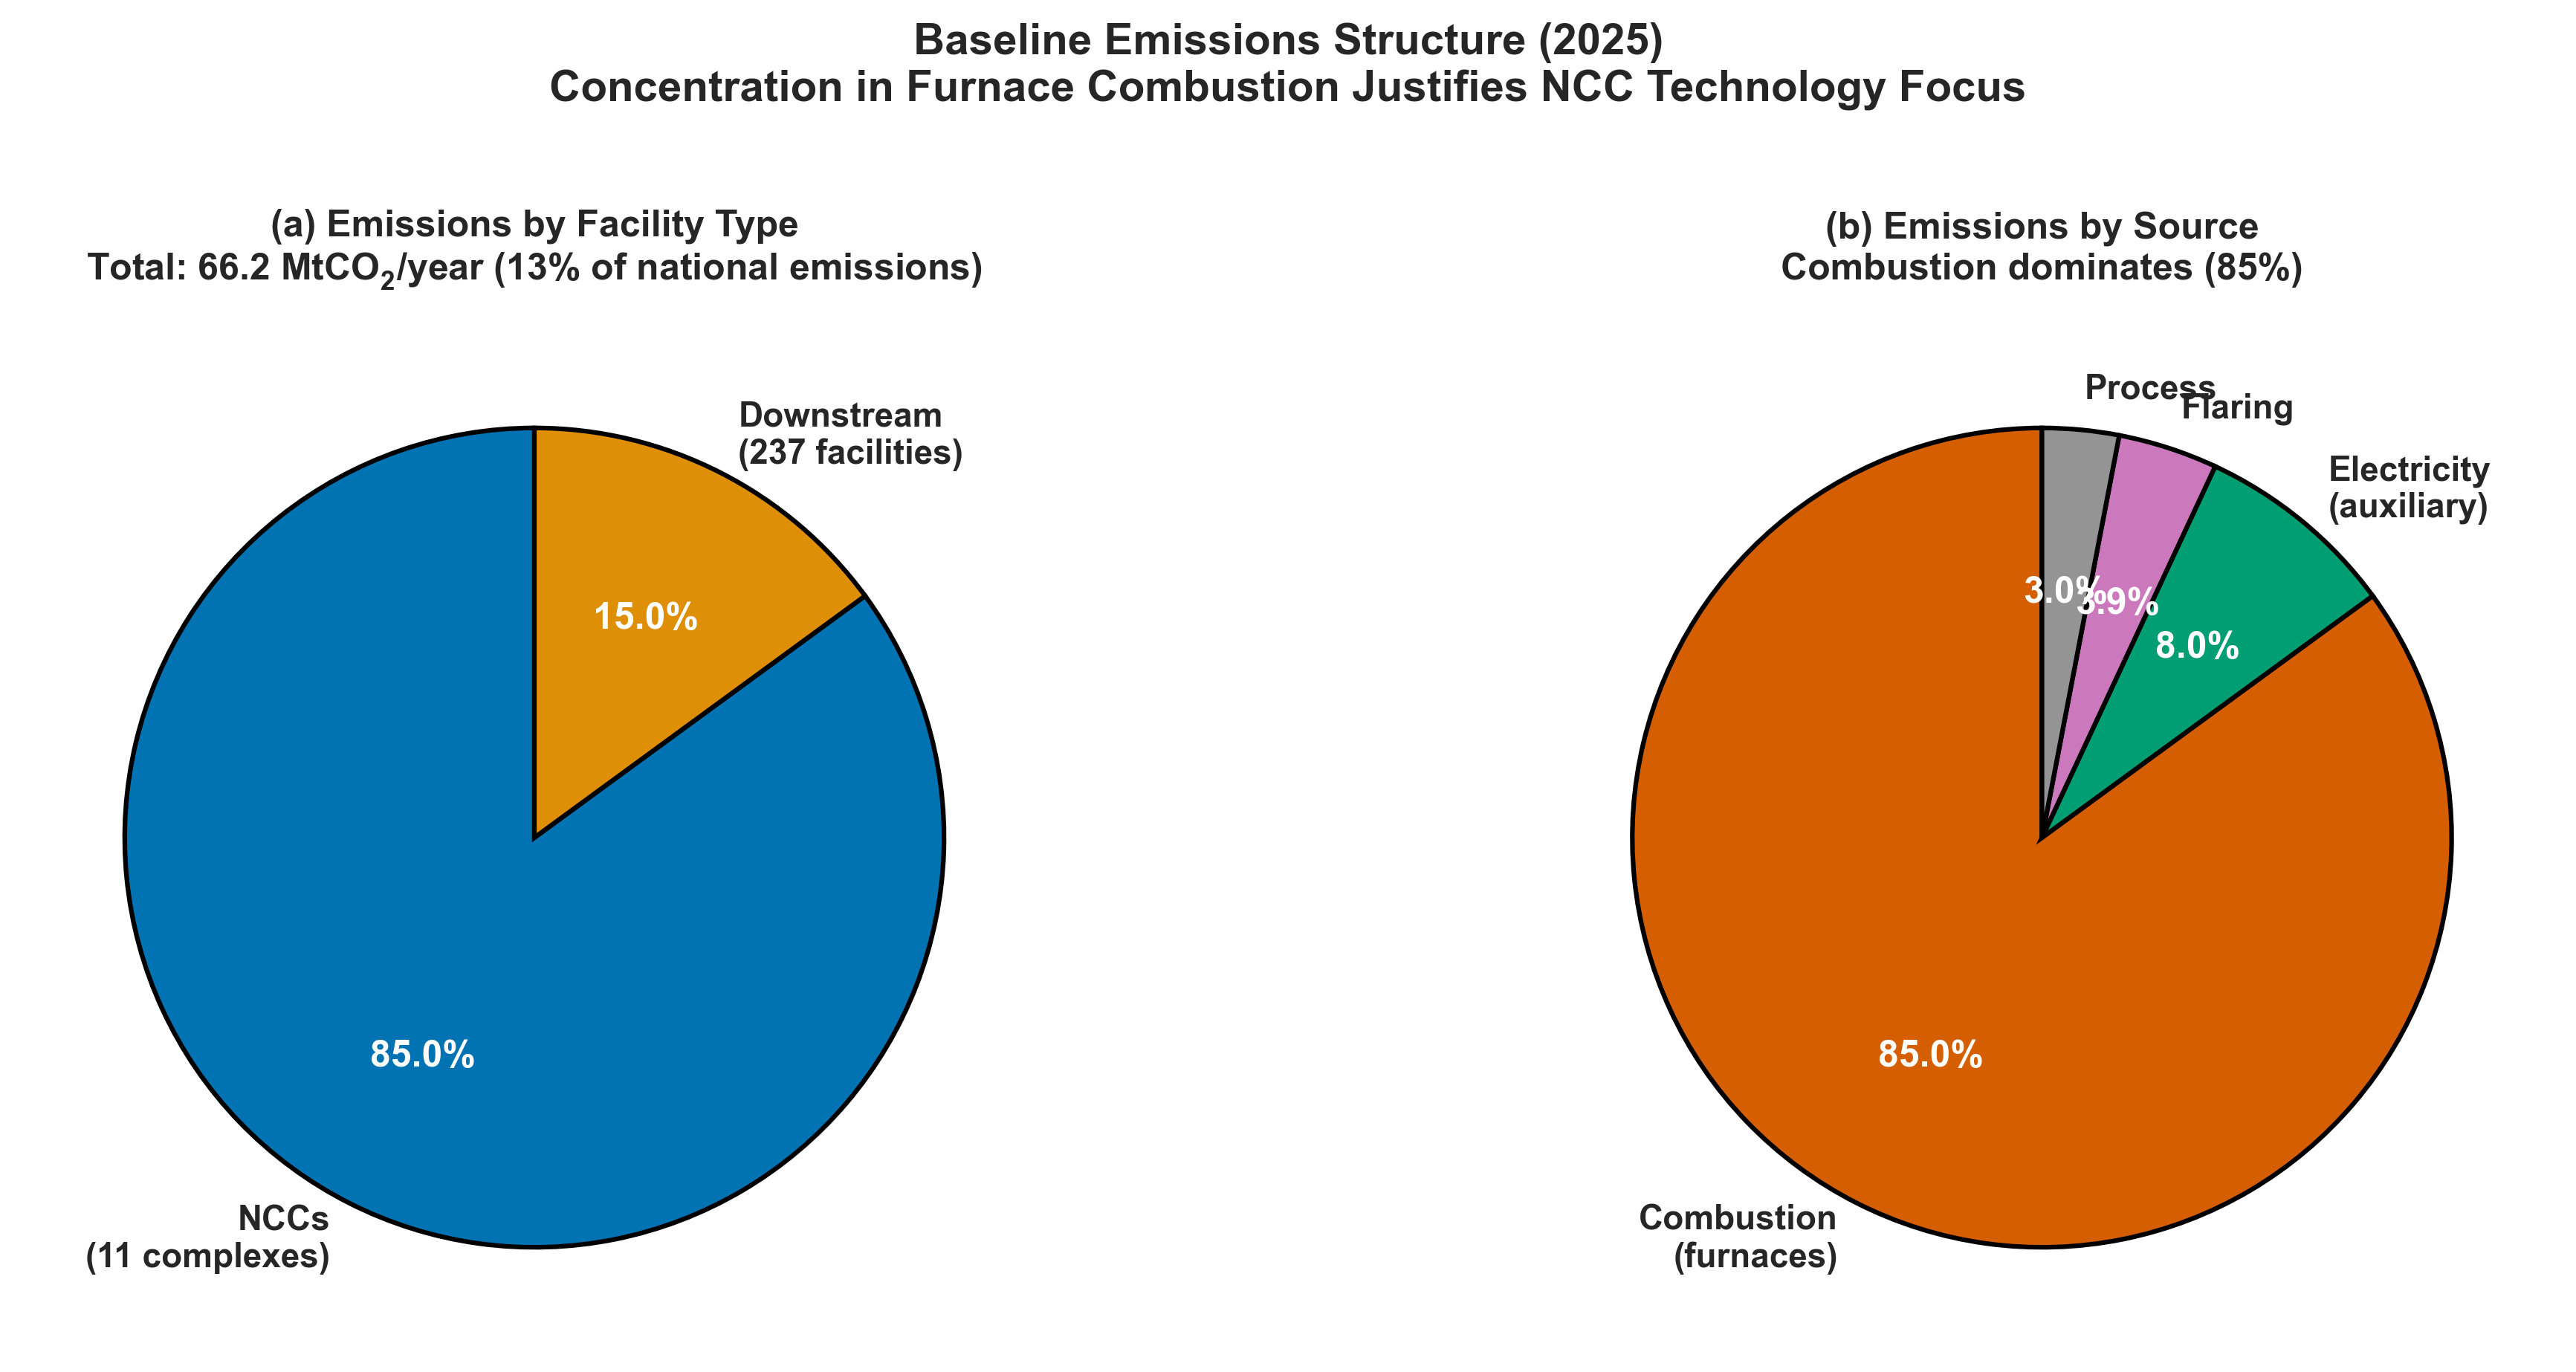
\includegraphics[width=0.85\textwidth]{figures_for_submission/figure7.png}
\caption{\textbf{Baseline Emissions Structure (2025).} Two-panel breakdown showing (a) emissions by facility type: NCCs 85\%, downstream 15\%; and (b) emissions by source: combustion 85\%, electricity 8\%, flaring 4\%, process 3\%. Total sector: 66.2 MtCO$_2$/yr (13\% of national emissions). Concentration in NCC combustion justifies focus on furnace decarbonization technologies. Created by author using facility-level MACC model.}
\label{fig:baseline}
\end{figure}

\subsection{Technology-Level Costs and Feasibility}

Figure~\ref{fig:costs} presents cumulative decarbonization costs (2025--2050) across all six scenarios. The most striking finding is the minimal cost difference between hydrogen and electricity technology pathways within each production scenario. For the Shaheen growth scenario, NCC-H\textsubscript{2} achieves cumulative costs of \$31.4 billion compared to \$33.3 billion for NCC-Electricity---a difference of only \$1.8 billion or 6\%. This pattern holds across production scenarios: 25\% restructuring shows \$15.1 billion (H\textsubscript{2}) versus \$16.7 billion (Electricity) (10\% difference), while 40\% restructuring yields \$13.0 billion versus \$14.5 billion (11\% difference).

The underlying MACC analysis (Figure~\ref{fig:macc}) reveals why these costs converge, though as discussed in Section~\ref{sec:discussion}, this cost similarity proves misleading for policy when energy system constraints are considered. Both pathways deploy identical supporting technologies---RE PPAs at \$20/tCO\textsubscript{2} and heat pumps at \$40/tCO\textsubscript{2}---for lower-cost abatement options. The primary NCC technologies show marginal costs of \$65/tCO\textsubscript{2} for H\textsubscript{2} versus \$72/tCO\textsubscript{2} for electricity in 2050 after learning effects. This 10\% technology cost difference translates to merely 6\% cumulative cost difference when integrated over the full deployment period. From a conventional MACC perspective emphasizing cost per ton of CO\textsubscript{2} abated, both pathways appear economically viable and would likely be deployed simultaneously absent other constraints.

In contrast, production pathway choice exerts far larger cost impacts. Comparing Shaheen to 40\% restructuring within the same technology route reveals cost differences of 58\% (\$31.4B to \$13.0B for H\textsubscript{2}; \$33.3B to \$14.5B for Electricity). Standard MACC analysis based solely on these cost metrics would conclude that both NCC-H\textsubscript{2} and NCC-Electricity pathways are economically viable, with choice between them potentially driven by minor differences in learning rate assumptions, fuel price trajectories, or investor preferences. However, this conclusion proves premature when energy system constraints are considered. Table~\ref{tab:scenarios} summarizes the complete six-scenario results.

\begin{figure}[htbp]
\centering
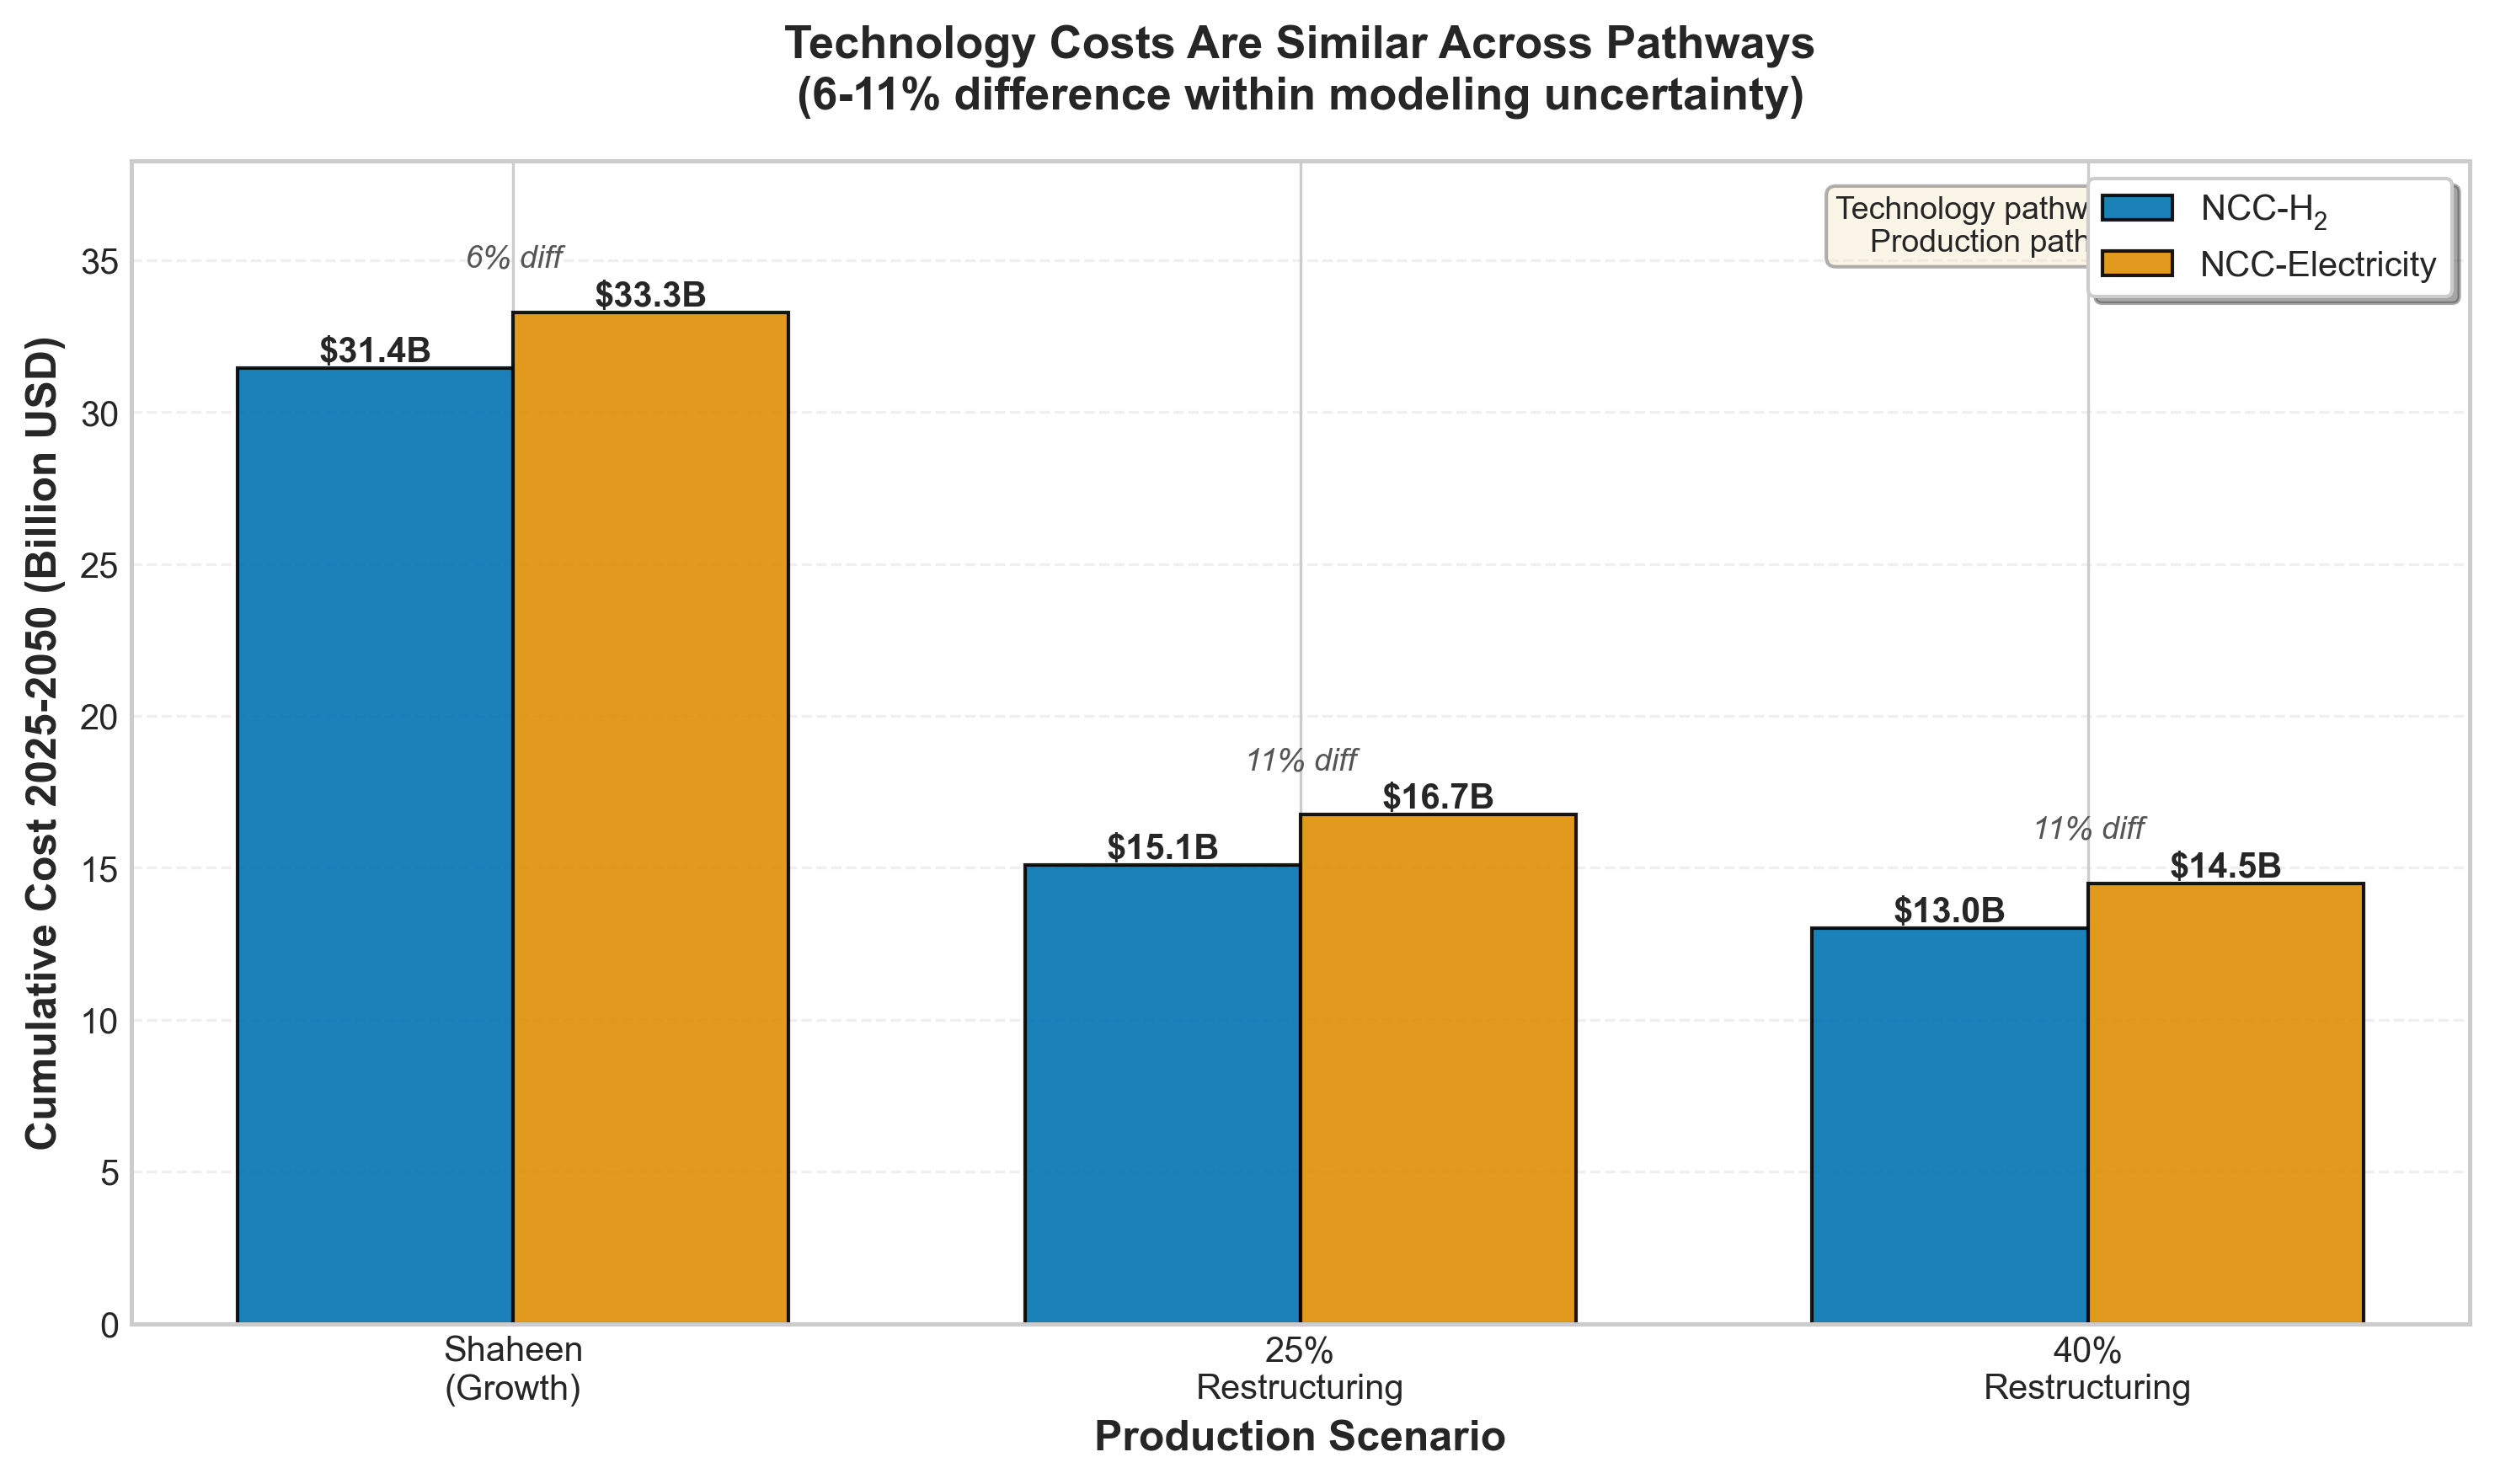
\includegraphics[width=0.95\textwidth]{figures_for_submission/figure1.png}
\caption{\textbf{Cumulative Decarbonization Costs Across Six Scenarios (2025-2050).} Bar chart showing technology pathway costs (H$_2$ vs Electricity) across three production scenarios. Technology choice shows 6-11\% cost variation while production pathway choice shows 58\% variation. Both technology pathways appear economically viable based on cost metrics, setting up the paradox where similar costs mask divergent energy demands. Created by author using facility-level MACC model.}
\label{fig:costs}
\end{figure}

\begin{table}[htbp]
\centering
\small
\caption{\textbf{Six-Scenario Results Summary (2050)}}
\label{tab:scenarios}
\begin{tabular}{@{}llcccc@{}}
\toprule
\textbf{Scenario} & \textbf{Technology} & \textbf{Cost} & \textbf{Reduction} & \textbf{H\textsubscript{2}} & \textbf{Electricity} \\
& \textbf{Pathway} & \textbf{(\$B)} & \textbf{(\%)} & \textbf{(Mt/yr)} & \textbf{(TWh/yr)} \\
\midrule
\multirow{2}{*}{Shaheen} & H\textsubscript{2} & 31.4 & 63 & 7.70 & 0.02 \\
& Electricity & 33.3 & 63 & 0.00 & 164.5 \\
\addlinespace
\multirow{2}{*}{25\% Restructure} & H\textsubscript{2} & 15.1 & 62 & 4.63 & 0.01 \\
& Electricity & 16.7 & 62 & 0.00 & 98.9 \\
\addlinespace
\multirow{2}{*}{40\% Restructure} & H\textsubscript{2} & 13.0 & 67 & 4.02 & 0.01 \\
& Electricity & 14.5 & 67 & 0.00 & 85.9 \\
\bottomrule
\end{tabular}
\begin{tablenotes}
\small
\item Technology pathway cost difference: 6--11\%. Production pathway cost difference: 58\% (Shaheen vs 40\% restructuring).
\end{tablenotes}
\end{table}

\begin{figure}[htbp]
\centering
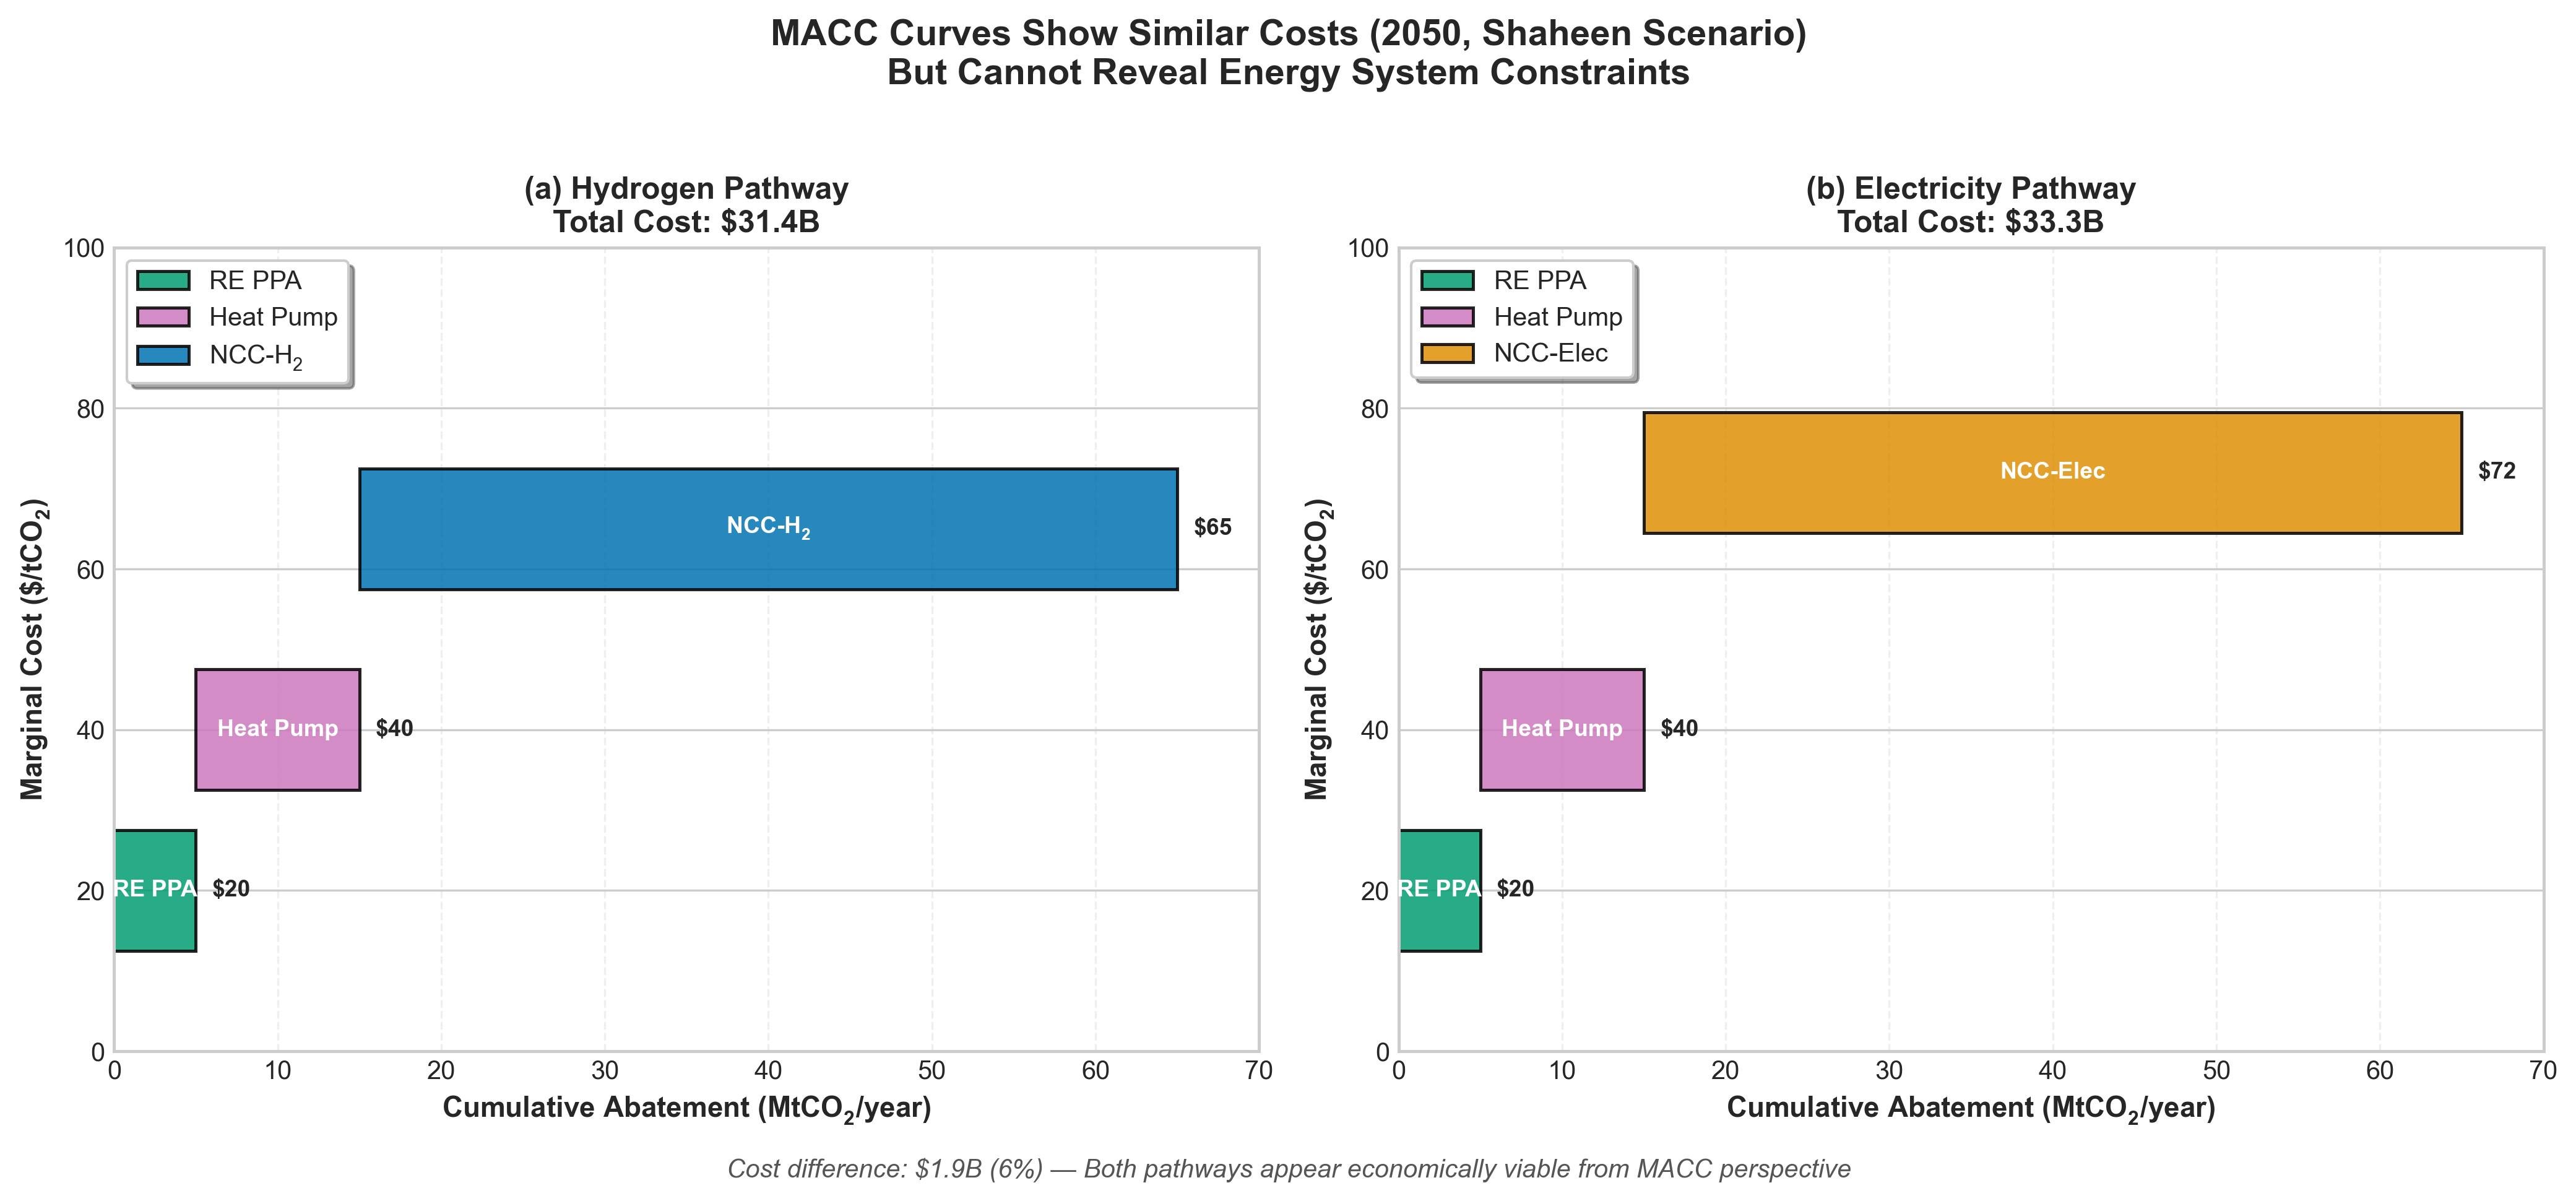
\includegraphics[width=0.95\textwidth]{figures_for_submission/figure3.png}
\caption{\textbf{MACC Comparison for Hydrogen and Electricity Pathways (2050).} Side-by-side comparison of marginal abatement cost curves for (a) hydrogen pathway (\$31.4B total) and (b) electricity pathway (\$33.3B total) in Shaheen scenario. Both show identical supporting technologies (RE PPA \$20/tCO$_2$, Heat Pumps \$40/tCO$_2$) with primary NCC technologies at \$65/tCO$_2$ (H$_2$) vs \$72/tCO$_2$ (Electricity). Conventional MACC analysis suggests both pathways viable, but cannot reveal energy system constraints. Created by author using facility-level MACC model.}
\label{fig:macc}
\end{figure}

\subsection{Energy System Constraints and Divergent Demands}

While technology costs remain comparable, energy system demands diverge dramatically between pathways (Figure~\ref{fig:electricity} and Figure~\ref{fig:hydrogen}). The Shaheen + NCC-Electricity scenario requires 164.5 TWh of additional annual electricity by 2050---representing 29.5\% of Korea's current total electricity consumption (558 TWh) and 96.8\% of the government's 2036 renewable electricity target (170 TWh). This demand arises exclusively from petrochemical sector decarbonization.

Conservative estimates of competing sectoral demands include electric vehicles (~40 TWh/year), building heat pumps (~30 TWh/year), steel sector (~50 TWh/year), and other industries (~30 TWh/year), totaling ~150 TWh/year. Under the Shaheen electricity pathway, petrochemical demand (164.5 TWh) exceeds all other competing sectors combined. Total incremental electricity demand would reach 314.5 TWh---equivalent to 56\% of Korea's current entire grid and 185\% of the 2036 renewable electricity target.

Even the 40\% restructuring scenario with electricity requires 85.9 TWh annually, equivalent to 15.4\% of current consumption and 50.5\% of the 2036 renewable target.

In stark contrast, the hydrogen pathway exhibits fundamentally different system integration characteristics. The Shaheen + NCC-H\textsubscript{2} scenario requires 7.7 million tons of H\textsubscript{2} annually by 2050, representing 27.6\% of Korea's Hydrogen Economy Roadmap supply target (27.9 Mt total: 3.0 Mt domestic plus 22.9 Mt imports). The 25\% restructuring scenario requires 4.6 Mt H\textsubscript{2} (16.6\% of target) while 40\% restructuring needs 4.0 Mt H\textsubscript{2} (14.4\% of target). All scenarios remain well within planned infrastructure capacity.

Critically, hydrogen infrastructure can be developed off-grid through dedicated renewable installations or via imports, avoiding competition for grid capacity. Korea's planned import strategy (22.9 Mt, 82\% of supply) reduces domestic renewable electricity requirements.

\begin{figure}[htbp]
\centering
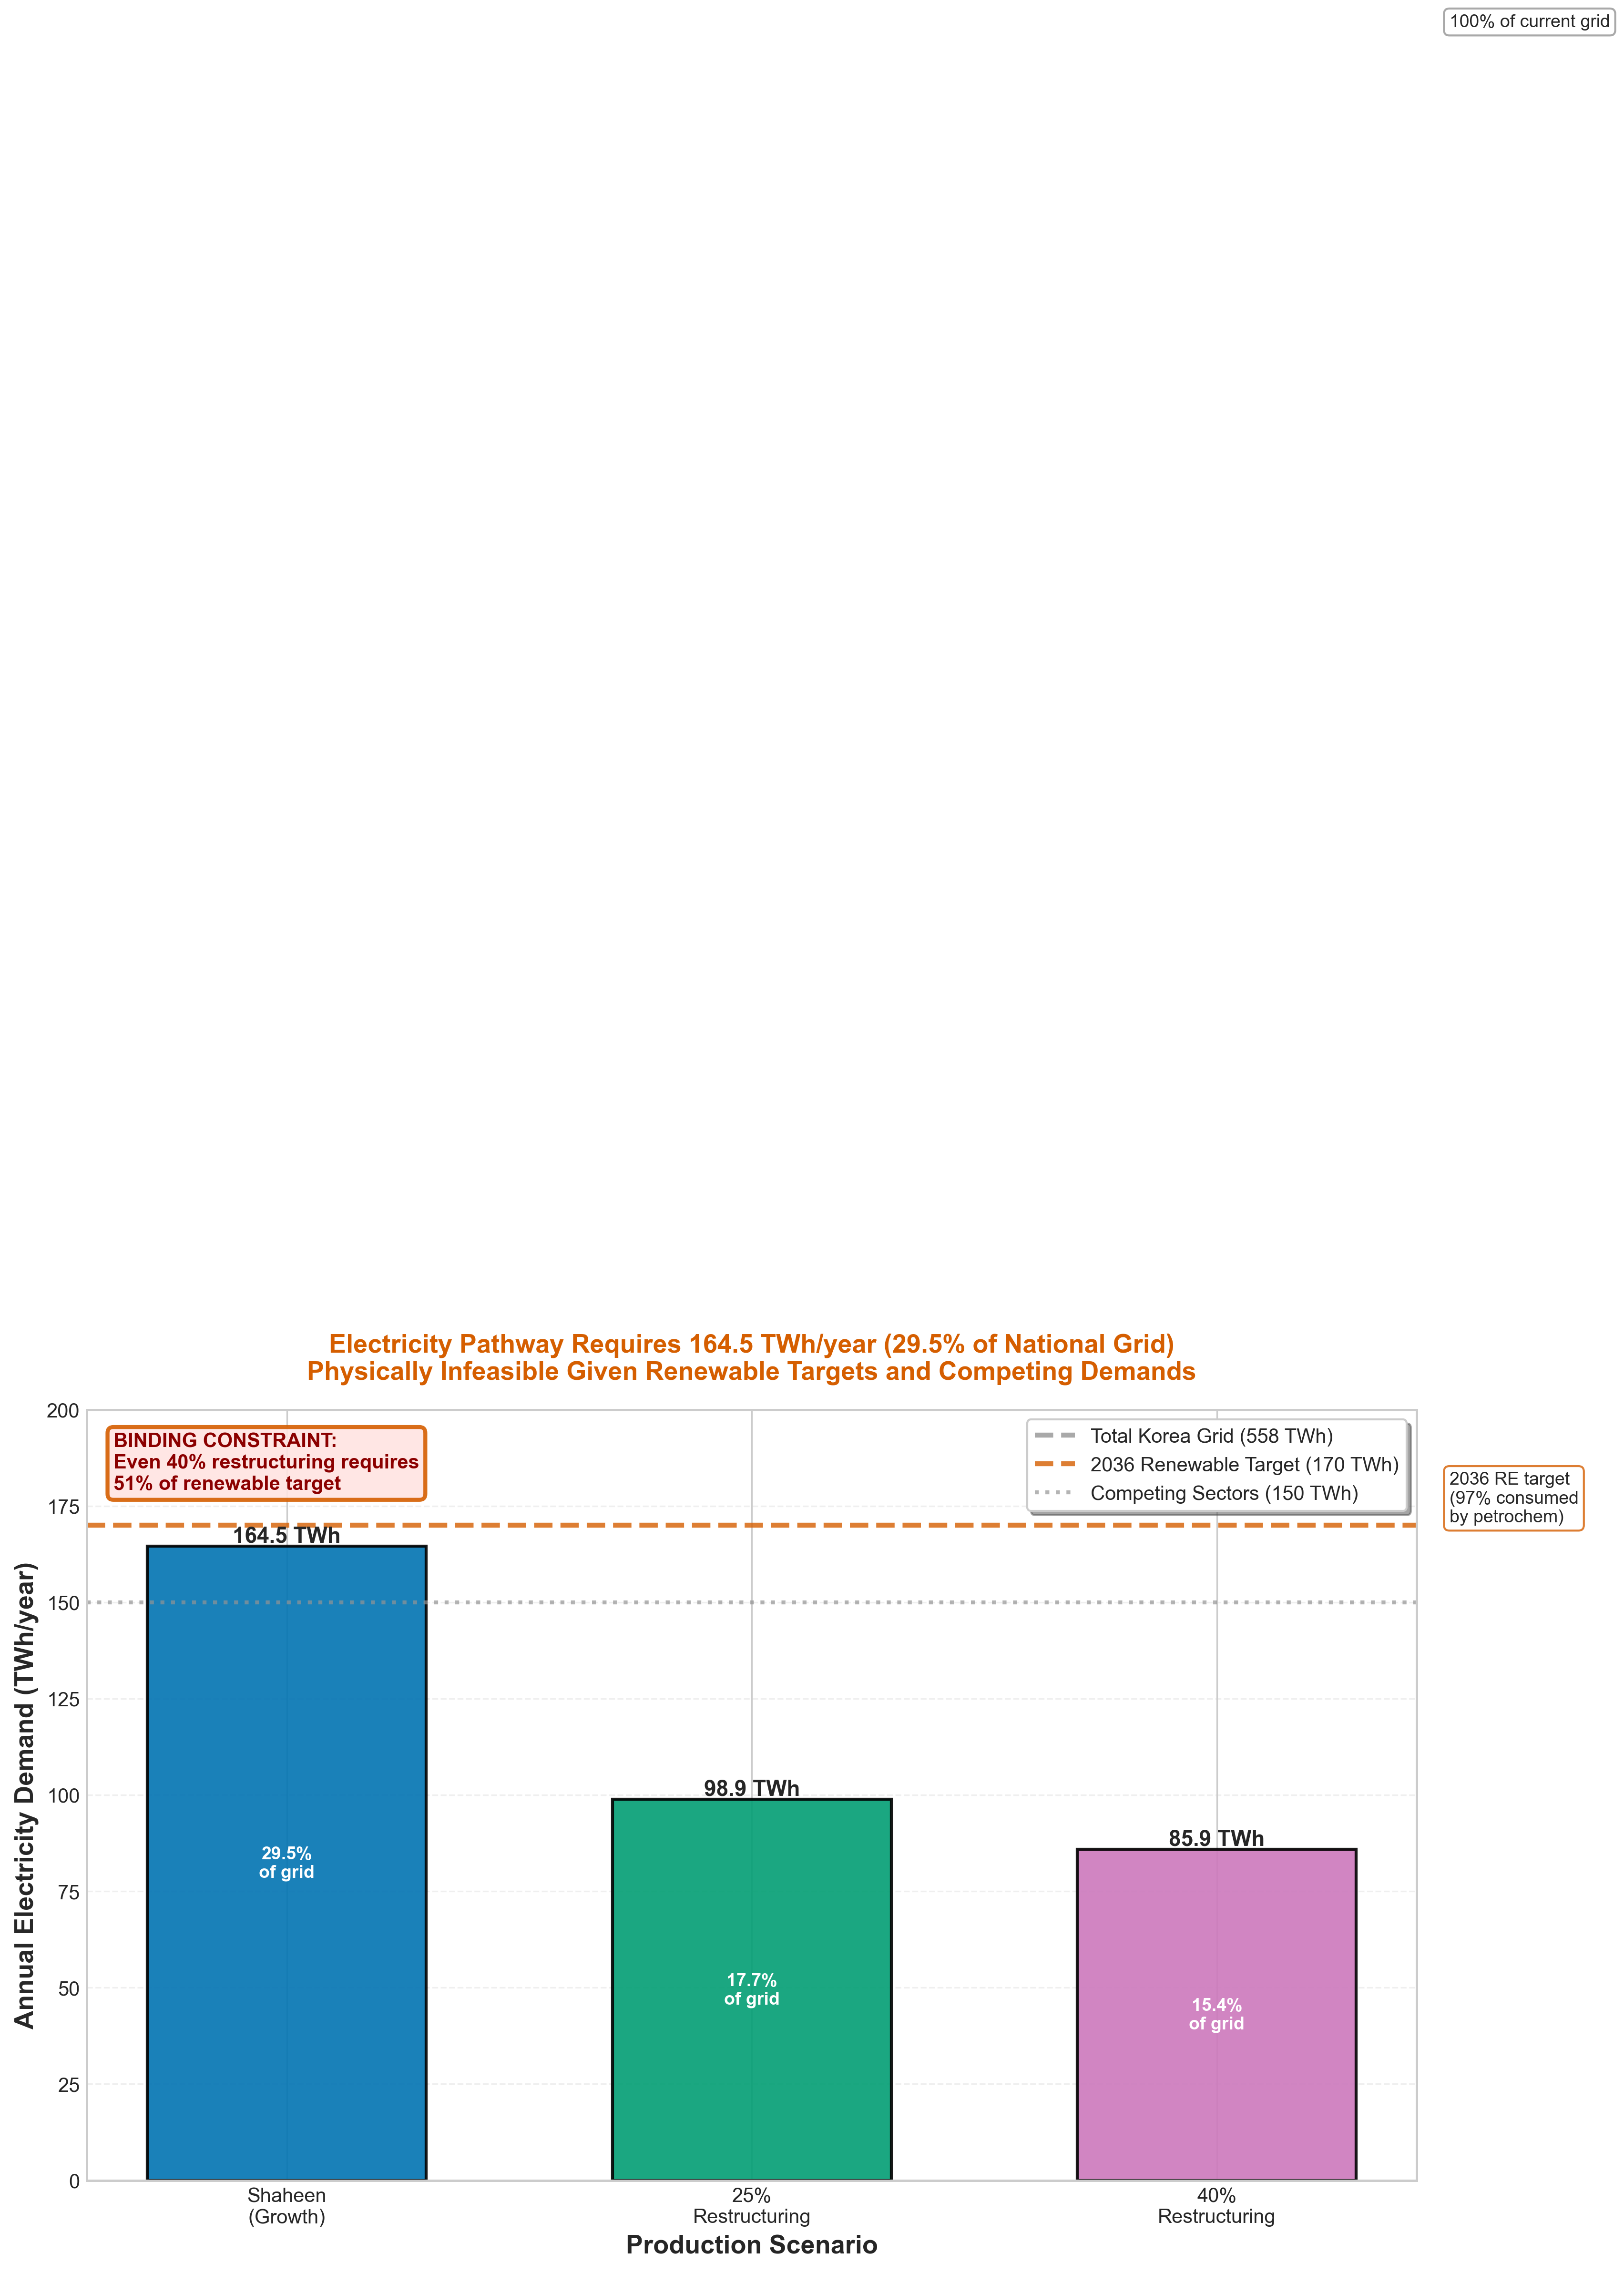
\includegraphics[width=0.95\textwidth]{figures_for_submission/figure4.png}
\caption{\textbf{Electricity Demand Requirements (2050).} Annual electricity demands by scenario: 164.5 TWh (Shaheen), 98.9 TWh (25\% restructuring), 85.9 TWh (40\% restructuring). Reference lines show Korea's grid (558 TWh), 2036 renewable target (170 TWh), and competing sectors (150 TWh). Shaheen pathway consumes 97\% of renewable target, rendering electricity pathway physically infeasible given competing sectoral demands. Created by author using facility-level MACC model.}
\label{fig:electricity}
\end{figure}

\begin{figure}[htbp]
\centering
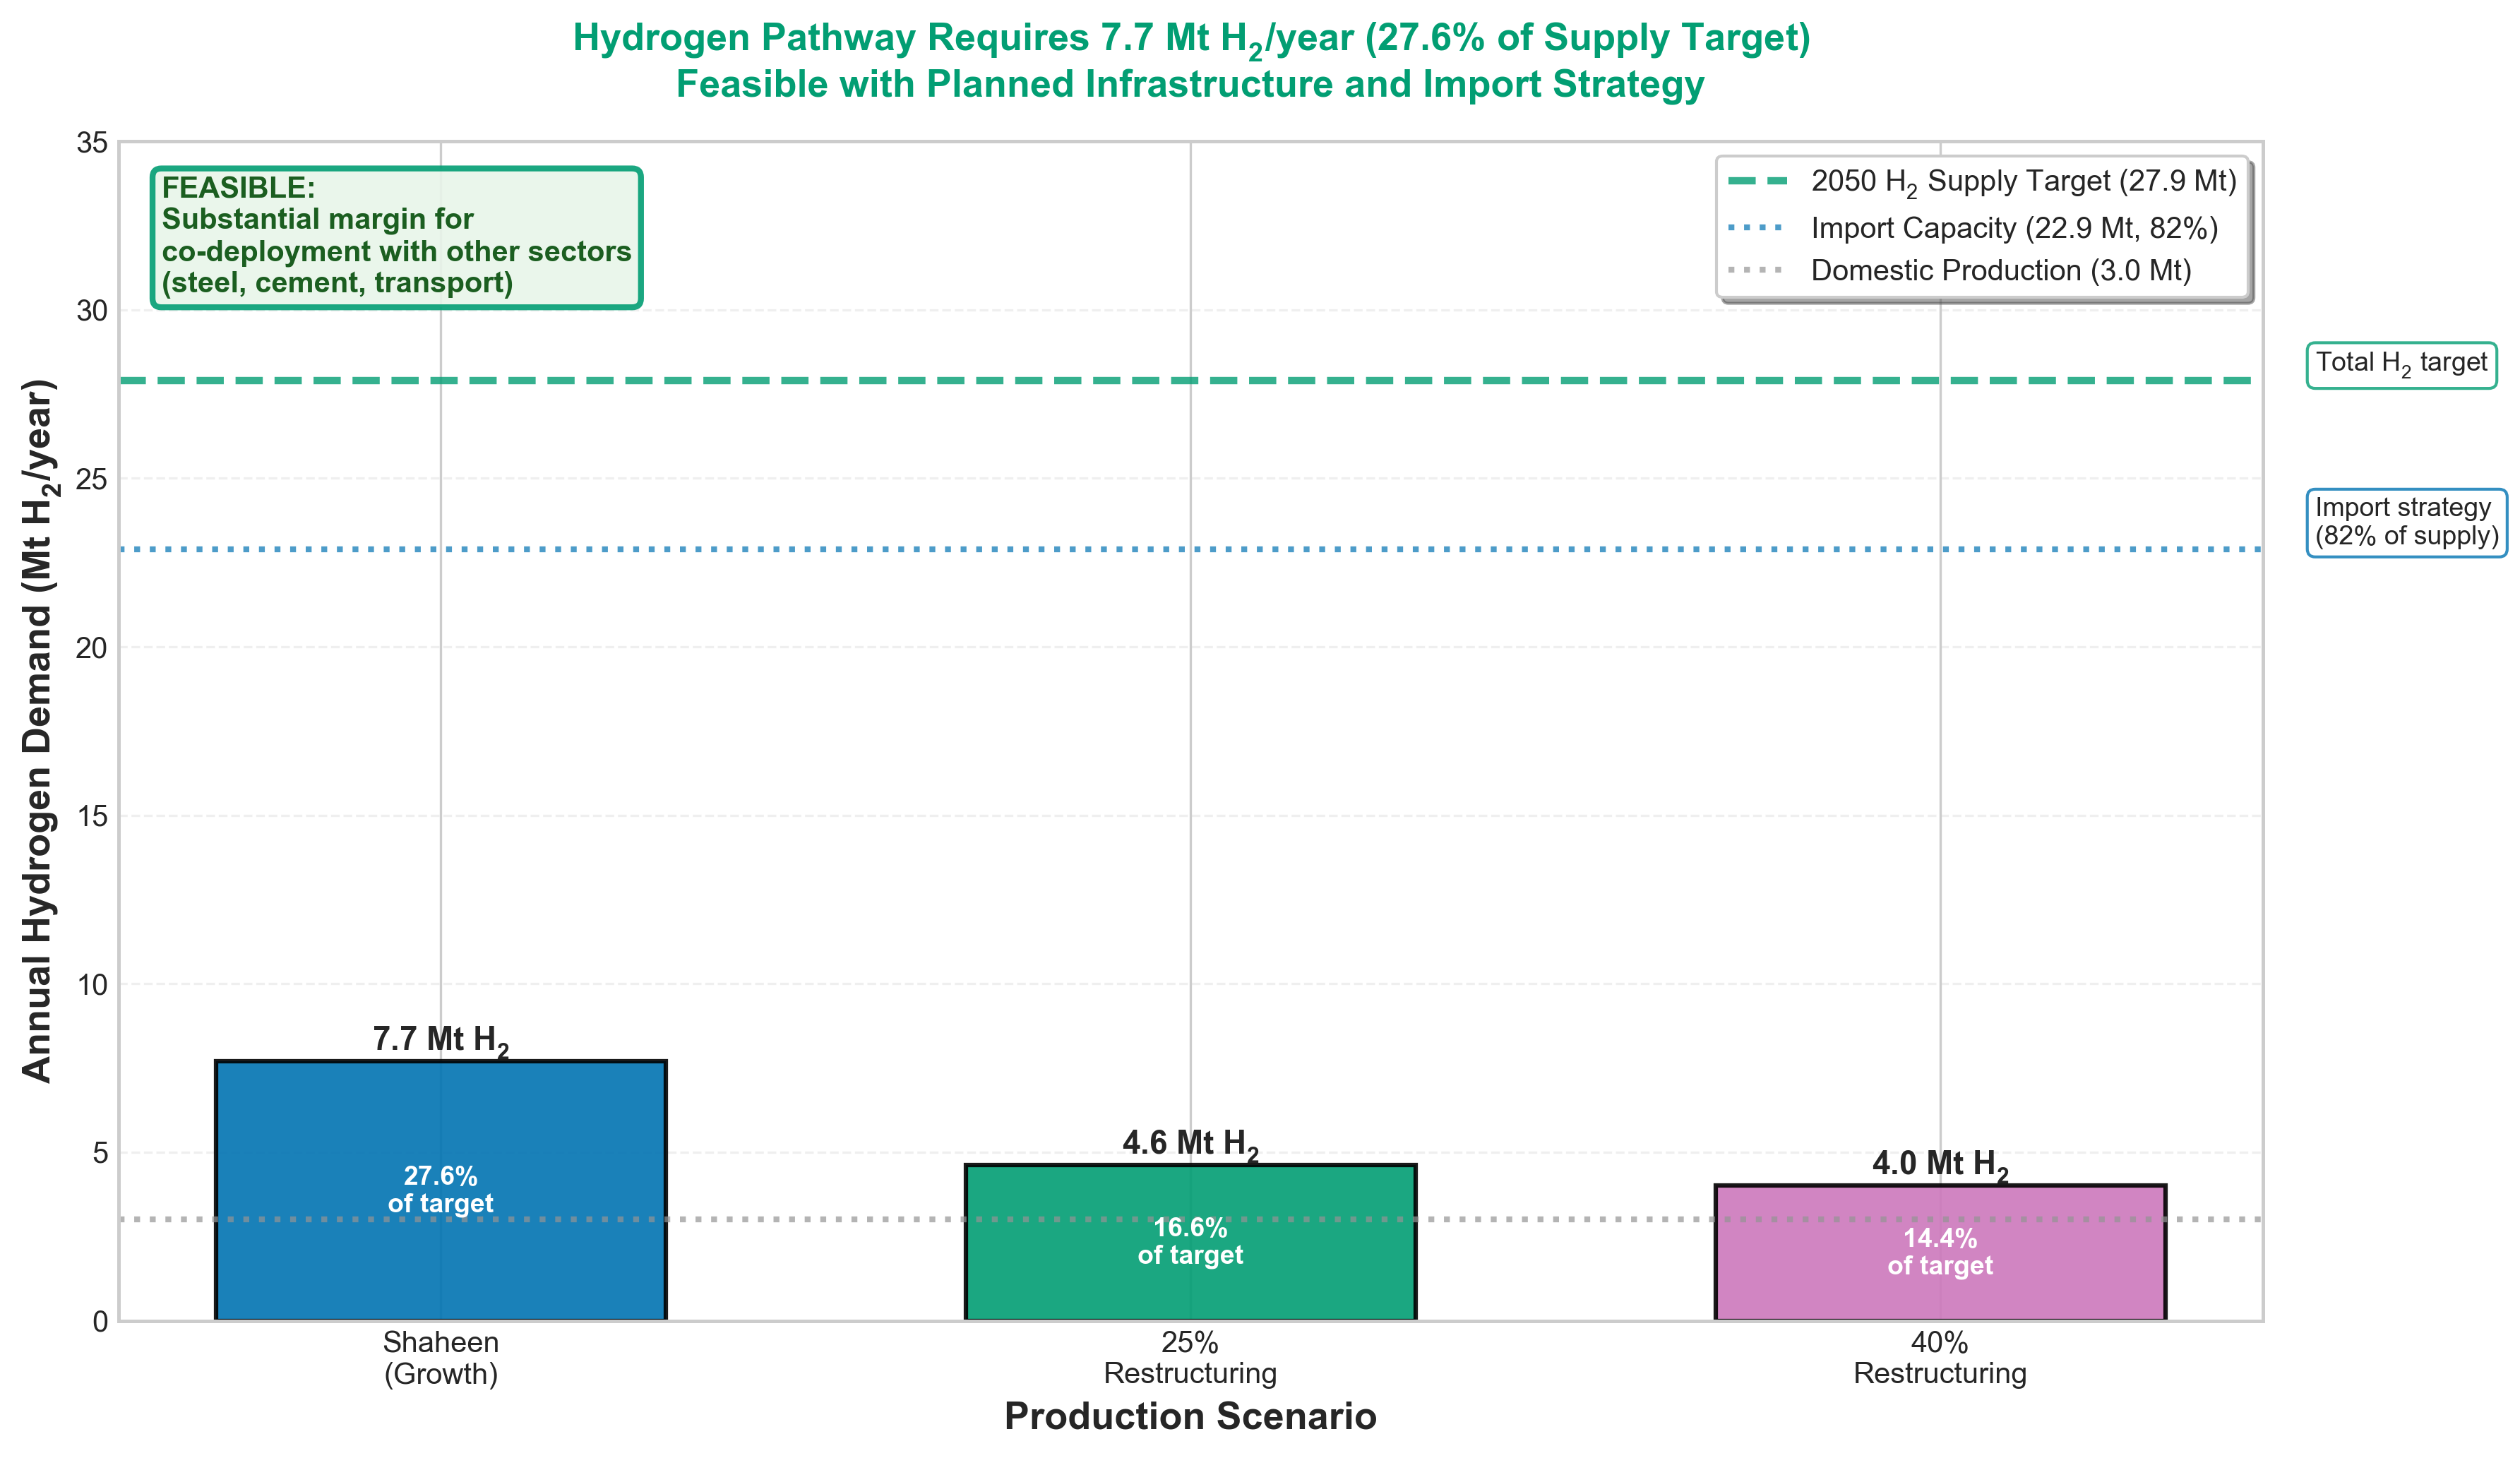
\includegraphics[width=0.95\textwidth]{figures_for_submission/figure5.png}
\caption{\textbf{Hydrogen Demand Requirements (2050).} Annual hydrogen demands by scenario: 7.7 Mt (Shaheen), 4.6 Mt (25\% restructuring), 4.0 Mt (40\% restructuring). Reference lines show Korea's H$_2$ targets: 27.9 Mt total supply (3.0 Mt domestic, 22.9 Mt imports). All scenarios remain within 14-28\% of supply target with substantial margin for co-deployment. Import strategy avoids grid constraints. Created by author using facility-level MACC model.}
\label{fig:hydrogen}
\end{figure}

\subsection{System-Level Feasibility Comparison}

The energy system demand analysis exposes a fundamental constraint invisible to conventional MACC methodology. While NCC-H\textsubscript{2} and NCC-Electricity appear similarly viable when evaluated solely on \$/tCO\textsubscript{2} metrics (6\% cost difference), system-level integration reveals that the electricity pathway is physically infeasible given Korea's renewable energy targets and competing sectoral demands. Even with aggressive capacity restructuring (40\% reduction), the electricity pathway would require 51\% of the 2036 renewable target. The hydrogen pathway aligns with policy targets, with petrochemical demand representing 14--28\% of planned supply depending on production scenario. Table~\ref{tab:feasibility} compares energy demands against Korea's policy targets, revealing the binding constraint.

\begin{table}[htbp]
\centering
\small
\caption{\textbf{Energy System Demands Against Korea Policy Targets}}
\label{tab:feasibility}
\begin{tabular}{@{}lccccc@{}}
\toprule
\textbf{Metric} & \textbf{Shaheen} & \textbf{25\% Rest.} & \textbf{40\% Rest.} & \textbf{Korea} & \textbf{Feasible?} \\
& & & & \textbf{Target} & \\
\midrule
\multicolumn{6}{l}{\textit{Electricity Pathway}} \\
Electricity (TWh/yr) & \textbf{164.5} & \textbf{98.9} & \textbf{85.9} & 170 (2036 RE) & \\
\% of Grid (558 TWh) & \textbf{29.5\%} & \textbf{17.7\%} & \textbf{15.4\%} & --- & \\
\% of RE Target & \cellcolor{red!20}\textbf{96.8\%} & \cellcolor{orange!20}\textbf{58.1\%} & \cellcolor{orange!20}\textbf{50.5\%} & 100\% & \cellcolor{red!20}\textbf{NO} \\
\addlinespace
\multicolumn{6}{l}{\textit{Hydrogen Pathway}} \\
H\textsubscript{2} (Mt/yr) & \textbf{7.70} & \textbf{4.63} & \textbf{4.02} & 27.9 (2050) & \\
\% of H\textsubscript{2} Target & \cellcolor{green!20}\textbf{27.6\%} & \cellcolor{green!20}\textbf{16.6\%} & \cellcolor{green!20}\textbf{14.4\%} & 100\% & \cellcolor{green!20}\textbf{YES} \\
\bottomrule
\end{tabular}
\begin{tablenotes}
\small
\item Competing sectoral electricity demands (~150 TWh): transport 40 TWh, buildings 30 TWh, steel 50 TWh, other industries 30 TWh. Electricity pathway consumes 51--97\% of renewable target for single sector before accounting for competing demands.
\end{tablenotes}
\end{table}

% Figures will be placed here - reference using \ref{fig:costs}, etc.
% Actual figures uploaded separately as per journal requirements

% Figure labels for cross-referencing:
% \label{fig:baseline}      - Figure 7: Baseline Emissions Structure
% \label{fig:costs}         - Figure 1: Cost Comparison
% \label{fig:macc}          - Figure 3: MACC Comparison (H2 vs Electricity)
% \label{fig:electricity}   - Figure 4: Electricity Demand
% \label{fig:hydrogen}      - Figure 5: Hydrogen Demand

\section{Discussion}
\label{sec:discussion}

\subsection{The Partial Equilibrium Trap}

Our results (Section~\ref{sec:results}) demonstrate a fundamental limitation of standard MACC methodology: partial equilibrium analysis that evaluates technologies in isolation systematically underestimates binding energy system constraints. The 6\% cost difference between pathways appears negligible when assessed individually. However, aggregating facility-level choices reveals that the electricity pathway requires 164.5 TWh annually---29.5\% of Korea's grid and 96.8\% of the renewable target. This demand magnitude transforms the pathway from ``slightly more expensive'' to ``physically infeasible.''

This extends recent critiques of MACC methodology \citep{Kesicki2021} beyond acknowledged limitations. Bataille et al. (2023) emphasize that net-zero pathways in OECD countries require system-level transformation rather than technology substitution, noting that ``inertia in energy systems creates binding constraints invisible to partial equilibrium models'' \citep{Bataille2023}. Fajardy \& Mac Dowell (2022) identify resource and integration limits as critical gaps in industrial hydrogen assessments, demonstrating that primary energy availability and infrastructure constraints can render apparently viable pathways infeasible at scale \citep{Fajardy2022}. Material Economics (2019, 2023) documents similar bottlenecks for EU industrial decarbonization, showing renewable electricity demands from heavy industry alone could exceed 1,200 TWh by 2050---equivalent to 40\% of total EU electricity consumption---creating fundamental allocation challenges between sectors \citep{MaterialEconomics2019,MaterialEconomics2023}. Kim et al. (2023) provide Korean context, arguing hydrogen infrastructure development represents necessary rather than optional investment for achieving carbon neutrality in heavy industry given Korea's resource constraints \citep{Kim2023}.

We demonstrate that even when methodological refinements are addressed, partial equilibrium frameworks systematically fail to identify capacity constraints emerging at the energy system level. The binding constraint is not technology cost but systemic integration---a dimension absent from conventional MACC analysis yet decisive for pathway feasibility. This aligns with Carbon Neutrality journal's emphasis on technology-system co-optimization: achieving net-zero requires configuring energy systems to accommodate sectoral demands, not merely selecting lowest-cost technologies in isolation.

The implications are profound. Studies concluding that ``electrification is cheaper than hydrogen'' based on technology-level analysis \citep{Diesing2025,Leicher2023} are correct in their domain but incomplete for policy. The relevant question is not which technology is cheaper per unit, but whether national energy systems can accommodate aggregate demands from sector-wide deployment---a question requiring explicit capacity assessment absent from partial equilibrium frameworks.

\subsection{Global Implications: Why This Matters Beyond Korea}

While our analysis focuses on South Korea, the fundamental constraint---that aggregate industrial electricity demands can exceed national renewable targets---applies universally to countries where grid growth faces physical, economic, or political limits. The pattern is remarkably consistent across industrialized economies with mature grids, limited renewable resources relative to industrial demands, and competing sectoral priorities.

\textbf{European Union}: The EU's industrial sector emits approximately 880 MtCO\textsubscript{2} annually across energy-intensive industries (steel, cement, chemicals, petrochemicals) \citep{MaterialEconomics2019}. If electrification pathway assumptions comparable to Korea's petrochemical sector apply proportionally, EU-wide industrial electrification could require 1,200--1,500 TWh annually---equivalent to 40--50\% of total EU electricity consumption (~3,000 TWh). This exceeds planned renewable capacity growth under REPowerEU (2030 target: 1,236 TWh renewable electricity, 45\% of consumption) \citep{EUREPowerEU2022}. The EU's Hydrogen Strategy targeting 20 Mt H\textsubscript{2} by 2030 (half imported) appears not aspirational but necessary given grid constraints.

\textbf{Japan}: Japan faces even more severe constraints than Korea---limited domestic renewable resources (mountainous terrain restricts onshore wind, limited suitable offshore wind areas), heavy industrial base (steel, chemicals, automotive), and mature grid infrastructure difficult to expand. Japan's Strategic Energy Plan already prioritizes hydrogen imports and ammonia co-firing for power generation \citep{JapanMETI2021}. Our findings suggest this hydrogen-centric strategy is necessary rather than optional, as electrifying Japan's industrial sector would likely require electricity volumes exceeding physically achievable renewable deployment given land constraints.

\textbf{China}: Despite being the world's largest industrial emitter (industrial sector: ~3.5 GtCO\textsubscript{2} annually) and largest renewable energy developer (wind and solar capacity growth exceeding all other countries combined), even China may face binding grid constraints if all industrial decarbonization routes through electrification. China's coal-dominated industrial regions (Hebei, Shanxi, Inner Mongolia) are geographically distant from renewable resources (western deserts, offshore wind). Long-distance transmission and grid integration costs could make dedicated hydrogen production and pipeline transport more feasible than grid electrification for heavy industry clusters.

The common thread: countries with resource constraints, mature grids, and large industrial bases cannot rely solely on electrification for industrial decarbonization. Hydrogen infrastructure becomes necessary infrastructure, not an optional premium pathway. This reframes hydrogen not as ``competitor'' to electrification but as ``complement''---essential for sectors where grid capacity constraints bind before technology costs do.

\subsection{Korea's Energy Policy: Validating the Hydrogen Strategy}

Our results provide quantitative validation for South Korea's Hydrogen Economy Roadmap, which has faced criticism as aspirational or economically inefficient compared to direct electrification. The Roadmap's 27.9 Mt H\textsubscript{2} target by 2050---with 82\% sourced via imports---appeared to many as an expensive detour given renewable electricity's declining costs. Our analysis reveals this strategy as necessary rather than optional, as quantified in Table~\ref{tab:feasibility}.

If petrochemical decarbonization pursued the electricity pathway, it would consume 96.8\% (Shaheen), 58.1\% (25\% restructuring), or 50.5\% (40\% restructuring) of the entire 2036 renewable increment. After accounting for competing demands (~150 TWh), total requirements (314.5 TWh under Shaheen) vastly exceed available supply.

The hydrogen strategy circumvents this bottleneck. By developing dedicated off-grid renewable installations or importing hydrogen produced using partner countries' resources, Korea can decarbonize heavy industry without competing for scarce grid capacity. The 82\% import share effectively accesses global renewable resources beyond Korea's domestic constraints.

Policy implications are immediate: (1) prioritize grid capacity for must-electrify sectors (transport, buildings) lacking alternatives; (2) accelerate hydrogen infrastructure (import terminals, pipelines, storage) with 10--15 year lead times; (3) enable off-grid renewable development bypassing grid connection requirements; (4) maintain technology-neutral incentives while recognizing system constraints guide aggregate outcomes.

\subsection{Production Pathway Effects}

Production pathway choice exerts an order of magnitude larger impact on total costs (58\% variation) than technology selection (6\% variation). The 40\% restructuring scenario reduces cumulative costs from \$31.4B to \$13.0B while cutting electricity demands from 164.5 TWh to 85.9 TWh---a 48\% reduction potentially moving from infeasible to marginally feasible territory.

This aligns with circular economy literature emphasizing demand-side interventions \citep{Kloo2024,EllenMacArthur2019,MaterialEconomics2019}. Strategies include enhanced recycling (targeting 30--40\% recycled content), material efficiency, bio-based substitution, and circular business models. However, demand-side interventions face severe political economy barriers: Korea's petrochemical industry employs over 100,000 workers directly, with regional economies heavily dependent on complex operations. Capacity reduction without managed transition creates concentrated losses while benefits disperse nationally, generating strong political resistance.

Effective strategies require integrating demand-side and supply-side interventions. Even ambitious technology deployment cannot fully resolve constraints under growth scenarios. Demand reduction creates ``policy space'' within energy system limits for deploying decarbonization technologies feasibly.

\subsection{Policy Implications for Carbon Neutrality}

Achieving carbon neutrality in energy-intensive industries requires reconciling technology costs with energy system capacity---a challenge this study quantifies explicitly. Our findings generate four immediate policy implications aligned with carbon neutrality pathways.

\textbf{First: Grid capacity emerges as the binding constraint, not technology cost.} The electricity pathway's 164.5 TWh demand consumes 97\% of Korea's 2036 renewable target for one sector alone. Adding competing demands from transport (40 TWh), buildings (30 TWh), steel (50 TWh), and other industries (30 TWh) produces total requirements of 314.5 TWh---185\% of the renewable target. This quantifies the infeasibility invisible to partial equilibrium MACC analysis. Grid-constrained countries must prioritize hydrogen infrastructure not as a premium option but as necessary infrastructure enabling industrial decarbonization without grid competition.

\textbf{Second: Hydrogen infrastructure becomes physically deployable where electrification fails.} The hydrogen pathway's 7.7 Mt H\textsubscript{2} demand represents only 28\% of Korea's 2050 supply target, leaving substantial margin for co-deployment across steel (estimated 2--3 Mt H\textsubscript{2}), cement (0.5 Mt), and transport (1--2 Mt). Import-based supply (22.9 Mt of 27.9 Mt total, 82\%) accesses global renewable resources beyond domestic grid constraints, enabling decarbonization without intersectoral competition. This validates hydrogen economy strategies in Japan, EU, and other resource-constrained economies as necessary rather than speculative \citep{Kim2023,Fajardy2022}.

\textbf{Third: Prioritize grid allocation for must-electrify sectors.} Transport and buildings lack viable alternatives to electrification at scale, while heavy industry can utilize hydrogen for high-temperature processes. Allocating Korea's 170 TWh 2036 renewable target requires explicit sectoral prioritization: transport electrification (40 TWh essential for air quality and oil import reduction), building heat pumps (30 TWh essential for heating decarbonization), grid decarbonization (baseload replacement), with residual capacity insufficient for petrochemical electrification (164.5 TWh required). Technology-system co-optimization demands strategic grid capacity allocation rather than assuming unlimited supply scalability.

\textbf{Fourth: Transitional and hybrid pathways warrant consideration.} While our analysis compares pure hydrogen and electricity pathways, practical deployment may involve transitional strategies: (1) \textit{Blue hydrogen with CCS}: utilizing existing natural gas infrastructure with carbon capture during the green hydrogen scale-up period (2025--2035), reducing upfront infrastructure investment while maintaining combustion experience; (2) \textit{Blended furnace systems}: gradual hydrogen blending (20--50--80\%) enabling incremental retrofits and operational learning before full conversion; (3) \textit{Partial electrification}: deploying heat pumps for auxiliary processes (150--200°C) while reserving hydrogen for high-temperature crackers (800--900°C), optimizing technology deployment by temperature range. These hybrid approaches merit systematic comparison in future work, balancing near-term feasibility with long-term carbon neutrality goals while managing infrastructure transition risks \citep{Bataille2023,MaterialEconomics2023}.

These implications reframe industrial decarbonization from technology selection to energy system architecture design. Carbon neutrality requires not identifying the cheapest technology per tCO\textsubscript{2} but configuring national energy systems to accommodate aggregate sectoral demands within infrastructure constraints---a planning challenge demanding technology-system co-optimization absent from current policy frameworks.

\subsection{Generalizability and Limitations}

While focused on South Korea, methodological insights likely generalize to other industrialized countries. The EU, Japan, and OECD countries exhibit comparable characteristics: limited domestic renewable resources relative to industrial demands, grid capacity constraints, and competing sectoral priorities. The binding constraint---that aggregate industrial electricity demands can exceed national renewable targets---applies wherever grid growth faces physical, economic, or political limits.

Our analysis employs simplifications warranting future research. First, we quantify electricity demands but do not model grid operations, transmission constraints, or temporal matching. Full grid modeling would provide higher resolution, though even simplified analysis reveals binding constraints at annual TWh levels. Second, we assume hydrogen supply meets demand at exogenous prices without modeling infrastructure development. Korea's strategy depends on import partnerships and shipping infrastructure subject to geopolitical uncertainties, though hydrogen demand (7.7 Mt) represents only 28\% of planned supply. Third, static optimization with annual time steps potentially misses dynamic effects such as investment timing and path dependencies. Fourth, our portfolio excludes carbon capture and storage, which faces challenges in Korea but warrants systematic comparison. Finally, Korea-specific parameters limit direct quantitative transferability, though the methodological contribution applies universally.

\subsection{Policy Recommendations}

Based on our findings, we recommend policymakers: (1) integrate energy system capacity assessment into industrial decarbonization planning, supplementing technology-level MACC with explicit aggregate demand calculations; (2) revise renewable targets to reflect true needs through transparent sectoral accounting; (3) prioritize hydrogen infrastructure for heavy industry given grid constraints; (4) reserve grid capacity for must-electrify sectors; (5) couple supply-side technology deployment with demand-side interventions, as circular economy policies create critical policy space within energy system constraints.

\section{Conclusion}

Partial equilibrium MACC analysis evaluates technologies in isolation without quantifying whether national energy systems can accommodate aggregate demands, producing systematically misleading pathway feasibility assessments. Through facility-level modeling of South Korea's 248 petrochemical facilities with explicit energy demand quantification, we demonstrate that hydrogen and electricity pathways show nearly identical costs (\$31.4B vs \$33.3B, 6\% difference) yet diverge by orders of magnitude in system integration: electricity requires 164.5 TWh annually (97\% of 2036 renewable target, physically infeasible), while hydrogen requires 7.7 Mt H\textsubscript{2} (28\% of 2050 target, deployable via off-grid production and imports). Methodologically, technology-system co-optimization must replace partial equilibrium analysis to avoid systematically underestimating binding capacity constraints. For carbon neutrality policy, our results validate hydrogen infrastructure as necessary rather than optional for heavy industry, with Korea's findings generalizing to EU, Japan, and resource-constrained OECD economies. Grid capacity, not technology cost, emerges as the binding constraint for industrial decarbonization---demanding explicit sectoral allocation rather than assuming unlimited renewable scalability. Achieving net-zero requires configuring national energy systems to accommodate aggregate sectoral demands within infrastructure constraints, not merely identifying lowest-cost technologies in isolation.

\section*{Declarations}

\subsection*{Availability of Data and Materials}

The MACC model code, input parameters, and scenario results are available on GitHub at \url{https://github.com/justjinsu/korea_petrochemical}. Facility-level emissions data are from Korea's National Greenhouse Gas Inventory (2022), available at \url{http://www.gir.go.kr}. All model outputs and supplementary data supporting the findings of this study are provided in supplementary materials and will be made publicly available upon publication.

\subsection*{Competing Interests}

The author declares no competing interests, financial or otherwise, that could inappropriately influence this work.

\subsection*{Funding}

This research received no specific grant from any funding agency in the public, commercial, or not-for-profit sectors. The research was conducted independently by the author.

\subsection*{Authors' Contributions}

JP conceived the study, developed the facility-level MACC model, conducted all analyses, and wrote the manuscript. The author read and approved the final manuscript.

\subsection*{Acknowledgements}

The author thanks the Korea Petrochemical Industry Association (KPIA) for publicly available production capacity data, and the Korea National Greenhouse Gas Inventory for facility-level emissions data. The author acknowledges the anonymous reviewers whose constructive feedback improved the manuscript.

\bibliographystyle{apalike}
\bibliography{references}

% Note: references.bib file should be created separately with BibTeX entries

\end{document}
